%File principale del documento su cui invocare la compilazione, vedi "istruzioni.txt" per più info

%Preambolo: la parte prima del \begin{document}
\documentclass[12pt,a4paper]{article} %formato del documento e grandezza caratteri

%Input del file metadata.tex della cartella locale "res/"
%lista di comandi presenti in template_latex.tex, da qui posso essere modificati secondo le esigenze

\newcommand{\DocTitle}{Verbale interno 2019-11-18} %variabile usata dal file template_latex.tex per settare il titolo del documento
%\newcommand{\DocAuthor}{Progetto "Predire in Grafana"} %variabile usata dal file template_latex.tex per settare l'autore del documento
\newcommand{\DocDate}{18 Novembre 2019} %variabile usata dal file template_latex.tex; Impostata manualmente, altrimenti ad ogni compilazione viene messa la data del giorno di compilazione.
\newcommand{\DocDesc}{Resoconto dell'incontro del gruppo \textit{VRAM Software} tenutosi in data 2019-11-18} %variabile usata dal file template_latex.tex per settare la descrizione del documento
\newcommand{\ver}{27.0.0} %variabile usata dal file template_latex.tex per settare la versione del documento
\newcommand{\app}{Toffoletto Massimo} %variabile usata dal file template_latex.tex per settare l'approvatore del documento
\newcommand{\red}{Dalla Libera Marco} %variabile usata dal file template_latex.tex per settare il redattore del documento
\newcommand{\test}{Schiavon Rebecca} %variabile usata dal file template_latex.tex per settare il verificatore del documento
\newcommand{\stat}{Approvato} %variabile usata dal file template_latex.tex per settare lo stato del documento
\newcommand{\use}{Interno} %variabile usata dal file template_latex.tex per indicare l'uso del documento %Contiene le varibili che descrivono il documento

%Input di file di configurazione presi dalla cartella "Template-LaTeX/config/", uguali per tutti i documenti
%Attenzione bisogna impostare il percorso del file!
% Tutti i pacchetti usati, da inserire nel preambolo prima delle configurazioni

\usepackage[T1]{fontenc} %Permette la sillabazione su qualsiasi testo contenente caratteri
\usepackage[utf8]{inputenc} %Serve per usare la codifica utf-8
\usepackage[english,italian]{babel} %Imposta italiano lingua principale, inglese secondaria. Es. serve per far apparire "indice" al posto di "contents"

\usepackage{graphicx} %Serve per includere le immagini

\usepackage[hypertexnames=false]{hyperref} %Gestisce i riferimenti/link. Es. Serve per rendere clickabili le sezioni dell'indice

\usepackage{float} %Serve per migliore la definizione di oggetti fluttuanti come figure e tabelle. Es. poter usare l'opzione [H] nelle figure ovvero tenere fissate le immagini che altrimenti LaTeX si sposta a piacere.

\usepackage{listings} %Serve per poter mettere snippets di codice nel testo

\usepackage{lastpage} %Serve per poter introdurre un'etichetta a cui si può fare riferimento Es. piè di pagina; poter fare " \rfoot{\thepage\ di \pageref{LastPage}} "

\usepackage{fancyhdr} %Per header e piè di pagina personalizzati

%Sono alcuni package che potranno esserci utili in futuro
%\usepackage{charter}
%\usepackage{eurosym}
\usepackage{subcaption}
%\usepackage{wrapfig}
%\usepackage{background}
\usepackage{longtable} % tabella che può continuare per più di una pagina
\usepackage[table]{xcolor} % ho dovuto aggiungere table in modo da poter colorare le row della tabella, dava: undefined control sequences
%\usepackage{colortbl}

\usepackage{dirtree} % usato per creare strutte tree-view in stile filesystem
\usepackage{xspace} % usato per inserire caratteri spazio
\usepackage[official]{eurosym}
\usepackage{pdflscape} %Inclusione pacchetti
% Configurazioni varie, da inserire nel preambolo dopo i pacchetti

\hypersetup{hidelinks} %serve per nascondere riquadri rossi che circondano i link 

\lstset{literate= {à}{{\`a}}1 } %Permette di usare lettere accentate nei listings

\pagestyle{fancy} %Imposto stile pagina
\fancyhf{} %Reset, se lo tolgo LaTex mette impostazioni di default (p.es numerazione pagine di default)


\lhead{
\includegraphics[scale=0.25]{img/logo_header.png}} %Left header che compare in ogni pagina
%\rhead{\leftmark} %Nome della top-level structure (p.es. Section in article o Chapter in book) in ogni pagina
\rhead{\DocTitle\ v. \ver} %Right header

\newcommand{\glo}{$_G$} %Comando per aggiungere il pedice G
\newcommand{\glosp}{$_G$ } %Comando per aggiungere il pedice G con spazio

\newcommand\Tstrut{\rule{0pt}{2.6ex}} % top padding
\newcommand\Bstrut{\rule[-0.9ex]{0pt}{0pt}} % bottom padding
\newcommand{\TBstrut}{\Tstrut\Bstrut} % top & bottom padding

%Setto il colore dei link
%\hypersetup{
%	colorlinks,
%	linkcolor=[HTML]{404040},
%	citecolor={purple!50!black},
%	urlcolor={blue!50!black}
%}

%Tabelle e tabulazione (può tornare utile)
%\setlength{\tablcolsep}{10pt}
%\renewcommand{\arraystretch}{1.4}

%Comando per aggiungere le pagine di ogni sezione
%\newcommand{\newSection}[1]{%
%	\input{res/sections/#1}
%}

% Comandi per aggiungere padding a parole contenute nella tabella; è una specie di strut (un carattere invisibile)
%\newcommand\Tstrut{\rule{0pt}{2.6ex}} % top padding
%\newcommand\Bstrut{\rule[-0.9ex]{0pt}{0pt}} % bottom padding
%\newcommand{\TBstrut}{\Tstrut\Bstrut} % top & bottom padding  %Configurazione pacchetti

\begin{document}
	%Input del file "frontmatter" preso dalla cartella "Template-LaTeX/config/", uguale per tutti i documenti
	%Attenzione bisogna impostare il percorso del file!
	% #### FRONTESPIZIO (frontmatter) ####
\setlength{\headheight}{33pt} %Distanzia l'header
\pagenumbering{gobble} %Toglie il numero di pagina
\begin{titlepage}
	\begin{center}
		
\includegraphics[scale=0.6]{img/logo.png} \\ %Logo
		\vspace{0.4cm} %Aggiunge uno spazio verticale di 0.5 cm
		
		{\LARGE Progetto "Predire in Grafana"} \\ %Nome progetto
		\vspace{0.4cm} %Attenzione a mettere il punto e NON la virgola
		
		{\Huge \textbf{\DocTitle}} \\ %Titolo, prende variabile definita in metadata.tex
		\vspace{0.4cm}
		
		\DocDate \\ %Data, prende variabile definita in metadata.tex
		\vspace{0.4cm}
		
		%Allineamento colonne: l=left r=right c=center, 
		%va specificato per ogni colonna
		%Se si vuole la riga tra colonne mettere "|"
		
		\begin{tabular}{r | l} %Elementi colonne separate da "&", le righe finiscono con "\\"
			Versione             & \ver \\
			Approvazione         & \app \\ 
			Redazione            & \red \\
			Verifica             & \test \\
			Stato                & \stat \\
			Uso                  & \use \\
		    Destinato a          & Zucchetti \\
						         & Prof. Vardanega Tullio\\
						         & Prof. Cardin Riccardo\\
			Email di riferimento & vram.software@gmail.com
		\end{tabular}
		\vfill
		\textbf{Descrizione} \\
		\DocDesc
	\end{center}
\end{titlepage}
\clearpage

% #### Impostazione header, footer  e numerazione pagine ####
\pagenumbering{arabic} %Pagine con i numeri arabi + reset a 1
\renewcommand{\footrulewidth}{0.4pt} %Di default footrulewidth==0 e quindi è invisibile, di default \headrulewith==0.4pt
\rfoot{\thepage\ di \pageref{LastPage}} %Pagina n di m, con numeri Arabi; usa il pacchetto "lastpage", in caso non sia possibile usare tale pacchetto mettere al fondo dell'ultima pagina "\label{LastPage}"

% #### Tabella dei log ####
% \textbf = grassetto; \Large = font più grande
% \rowcolors{quanti colori alternare}{colore numero riga pari}{colore numero riga dispari}: colori alternati per riga
% \rowcolor{color}: cambia colore di una riga
% p{larghezza colonna}: p è un tipo di colonna di testo verticalmente allineata sopra, ci sarebbe anche m che è centrata a metà ma non è precisa per questo utilizzo TBStrut; la sintassi >{\centering} indica che il contenuto della colonna dovrà essere centrato
% \TBstrut fa parte di alcuni comandi che ho inserito in config.tex che permetto di aggiungere un po' di padding al testo
% \\ [2mm] : questra scrittura indica che lo spazio dopo una break line deve essere di 2mm
% 

%\setcounter{secnumdepth}{0}
%\hfill \break
%\textbf{\Large{Diario delle modifiche}} \\


\addtocontents{toc}{\protect\setcounter{tocdepth}{0}} %Inserire questo per escludere una sezione dall'indice.

\section*{Registro delle modifiche} %Asterisco per fare sezione non numerata
\rowcolors{2}{gray!25}{gray!15}
\begin{longtable} {
		>{\centering}p{17mm} 
		>{\centering}p{19.5mm}
		>{\centering}p{24mm} 
		>{\centering}p{24mm} 
		>{}p{32mm}}
	\rowcolor{gray!50}
	\textbf{Versione} & \textbf{Data} & \textbf{Nominativo} & \textbf{Ruolo} & \textbf{Descrizione} \TBstrut \\
	14.7.0 & 2020-04-09 & Stantagiuliana Vittorio, Toffoletto Massimo e Spreafico Alessandro & \textit{Progettista}, \textit{Verificatore} e \textit{Responsabile di progetto} & Stesura, verifica e approvazione documento. \TBstrut \\ [2mm]
\end{longtable}

\addtocontents{toc}{\protect\setcounter{tocdepth}{4}} %Inserire questo per ripristinare il normale inserimento delle sezioni nell'indice. 4 significa fino al paragrah
\clearpage

% #### INDICE (tableofcontents) ####
\tableofcontents %Provoca la stampa dell'indice
\clearpage

\setcounter{secnumdepth}{4} %Permette di andare fino alla profondità del paragraph con la numerazione delle sezioni %Imposta il frontespizio, l'indice, header e footer
	
	
	
	%Tutte le sezioni del documento
	%\input{res/inserire nome sezione 1} 
	% ...
	%Mettere al suo interno una suddivisione con i 4 periodi che corrispondono alle scadenze. Per ognuno suddividere ulteriormente in periodi di analisi da definire. Alla fine di ognuno dei 4 periodi principali(delle 4 scadenze) fare un Gantt
%per ogni attività bisogna trovare un sottoperiodo e per ognuno un grafico di Gantt
\section{Pianificazione} 
Il nostro gruppo, per rispettare le scadenze elencate nella sezione \textit{Calendario delle attività}, ha deciso di suddividere lo sviluppo del prodotto\glosp e della sua documentazione nelle seguenti quattro attività:
\begin{itemize}
	\item analisi dei requisiti;
	\item progettazione\glosp architetturale;
	\item progettazione\glosp di dettaglio e codifica;
	\item validazione\glosp e collaudo.
\end{itemize}
La pianificazione ha lo scopo di gestire lo sviluppo del progetto\glosp suddividendolo in attività che, singolarmente, risultano più facili da realizzare. Per descrivere ogni attività, abbiamo deciso di suddividerle ulteriormente in periodi e abbiamo elencato i ruoli attivi durante lo svolgimento di ciascuno di essi.

\subsection{Analisi dei requisiti}
L'analisi dei requisiti è il primo macro periodo: inizia il 2019-11-14, giorno successivo alla formazione dei gruppi e termina il 2020-01-20, giorno precedente alla presentazione del progetto\glo. Durante questo macro periodo ci occuperemo principalmente dell'analisi di tutte le informazioni riguardanti il prodotto\glosp che dobbiamo sviluppare, l'organizzazione delle attività e la suddivisione delle risorse.

\subsubsection{Ruoli attivi}
\begin{itemize}
	\item Responsabile di progetto\glo;
	\item amministratore di progetto\glo;
	\item analista;
	\item progettista;
	\item verificatore.
\end{itemize}

\subsubsection{Periodi}
Abbiamo suddiviso il macro periodo della Analisi dei Requisiti nei seguenti sei periodi:
\paragraph*{I periodo: dal 2019-11-14 al 2019-11-27}
\begin{itemize}
	\item \textbf{Discussione dei capitolati}\glo: discussione interna, analizzando i fattori positivi e negativi di ogni capitolato\glo, per indirizzarci alla scelta di quale progetto\glosp realizzare;
	\item \textbf{Normazione}: discussione interna in merito alle regole da seguire per lo sviluppo della documentazione del progetto\glo. Iniziato il documento interno \textit{Norme di Progetto} nelle sue sezioni riguardanti: \textit{Studio di Fattibilità}, strumenti da utilizzare, documentazione, gestione della configurazione, processo\glosp di verifica e processi\glosp organizzativi;
	\item \textbf{Ricerca di strumenti e tecnologie}: inizio della ricerca di gruppo e individuale su strumenti e tecnologie necessari allo sviluppo della documentazione del progetto\glo;
	\item \textbf{Definizione dei ruoli}: suddivisione dei ruoli per le attività prese in considerazione; 
	\item \textbf{Pianificazione delle attività}: gestione delle risorse disponibili, suddivisione e pianificazione di tutte le attività che devono essere svolte in questo periodo;
	\item \textbf{Verifica}: attività di controllo dei documenti realizzati durante questo periodo.
\end{itemize}

\paragraph*{II periodo: dal 2019-11-28 al 2019-12-08}
\begin{itemize}
	\item \textbf{Studio di Fattibilità}: formalizzazione della scelta del capitolato\glosp con la stesura del documento \textit{Studio di Fattibilità v. 1.1.1};
	\item \textbf{Normazione}: revisione e aggiornamento delle \textit{Norme di Progetto} riguardanti \textit{Studio di Fattibilità} e strumenti da utilizzare;
	\item \textbf{Ricerca di strumenti e tecnologie}: continuazione della ricerca di strumenti e tecnologie da utilizzare per lo sviluppo del prodotto\glo;
	\item \textbf{Definizione dei ruoli}: suddivisione dei ruoli per le attività prese in considerazione; 
	\item \textbf{Pianificazione delle attività}: gestione delle risorse disponibili, suddivisione e pianificazione di tutte le attività che devono essere svolte in questo periodo;
	\item \textbf{Verifica}: attività di controllo dei documenti realizzati durante questo periodo.
\end{itemize}

\paragraph*{III periodo: dal 2019-12-09 al 2020-12-22}
\begin{itemize}
	\item \textbf{Normazione}: revisione e aggiornamento delle \textit{Norme di Progetto} riguardanti \textit{Analisi dei Requisiti}, \textit{Piano di Progetto} e strumenti da utilizzare;
	\item \textbf{Ricerca di strumenti e tecnologie}: continuazione della ricerca di strumenti e tecnologie da utilizzare per lo sviluppo del prodotto\glo;
	\item \textbf{Pianificazione delle attività}: gestione delle risorse disponibili, suddivisione e pianificazione di tutte le attività che devono essere svolte in questo periodo;
	\item \textbf{Analisi dei requisiti}: individuazione dei requisiti del prodotto\glosp in seguito a: incontri interni, analisi dei casi d'uso\glo, analisi del capitolato\glosp e incontro esterno col proponente.
	\item \textbf{Verifica}: attività di controllo dei documenti realizzati durante questo periodo.
\end{itemize}

\paragraph*{IV periodo: dal 2019-12-23 al 2020-01-01}
\begin{itemize}
	\item \textbf{Normazione}: revisione e aggiornamento delle \textit{Norme di Progetto} riguardanti \textit{Analisi dei Requisiti}, \textit{Piano di Qualifica}, gestione della qualità e strumenti da utilizzare;
	\item \textbf{Gestione della qualità}: inizio della discussione interna in merito a come definire e mantenere uno standard per garantire la qualità di tutti i documenti realizzati;
	\item \textbf{Ricerca di strumenti e tecnologie}: continuazione della ricerca di strumenti e tecnologie da utilizzare per lo sviluppo del prodotto\glo;
	\item \textbf{Pianificazione delle attività}: gestione delle risorse disponibili, suddivisione e pianificazione di tutte le attività che devono essere svolte in questo periodo;
	\item \textbf{Definizione dei casi d'uso}: realizzazione dei casi d'uso\glosp del prodotto\glosp richiesto dal proponente;
	\item \textbf{Verifica}: attività di controllo dei documenti realizzati durante questo periodo.
\end{itemize}


\paragraph*{V periodo: dal 2020-01-02 al 2020-01-14}
\begin{itemize}
	\item \textbf{Normazione}: revisione e aggiornamento delle \textit{Norme di Progetto} riguardanti: \textit{Piano di Qualifica}, \textit{Piano di Progetto} e strumenti da utilizzare;
	\item \textbf{Gestione della qualità}: individuazione di regole e metodi per mantenere e garantire la qualità del prodotto\glo;
	\item \textbf{Ricerca di strumenti e tecnologie}: continuazione della ricerca di strumenti e tecnologie da utilizzare per lo sviluppo del prodotto\glo;
	\item \textbf{Pianificazione delle attività}: gestione delle risorse disponibili, suddivisione e pianificazione di tutte le attività che devono essere svolte in questo periodo;
	\item \textbf{Analisi dei rischi}: discussione interna dei possibili rischi nella realizzazione del progetto\glo;
	\item \textbf{Stesura lettera di presentazione}: stesura della \textit{Lettera di Presentazione} in cui si propone una soluzione alla richiesta del proponente;
	\item \textbf{Verifica}: attività di controllo dei documenti realizzati durante questo periodo.
\end{itemize}

\paragraph*{VI periodo: dal 2020-01-15 al 2020-01-20}
\begin{itemize}
	\item \textbf{Preparazione alla discussione}: realizzazione della presentazione e preparazione individuale e di gruppo alla discussione.
\end{itemize}

\begin{figure}
	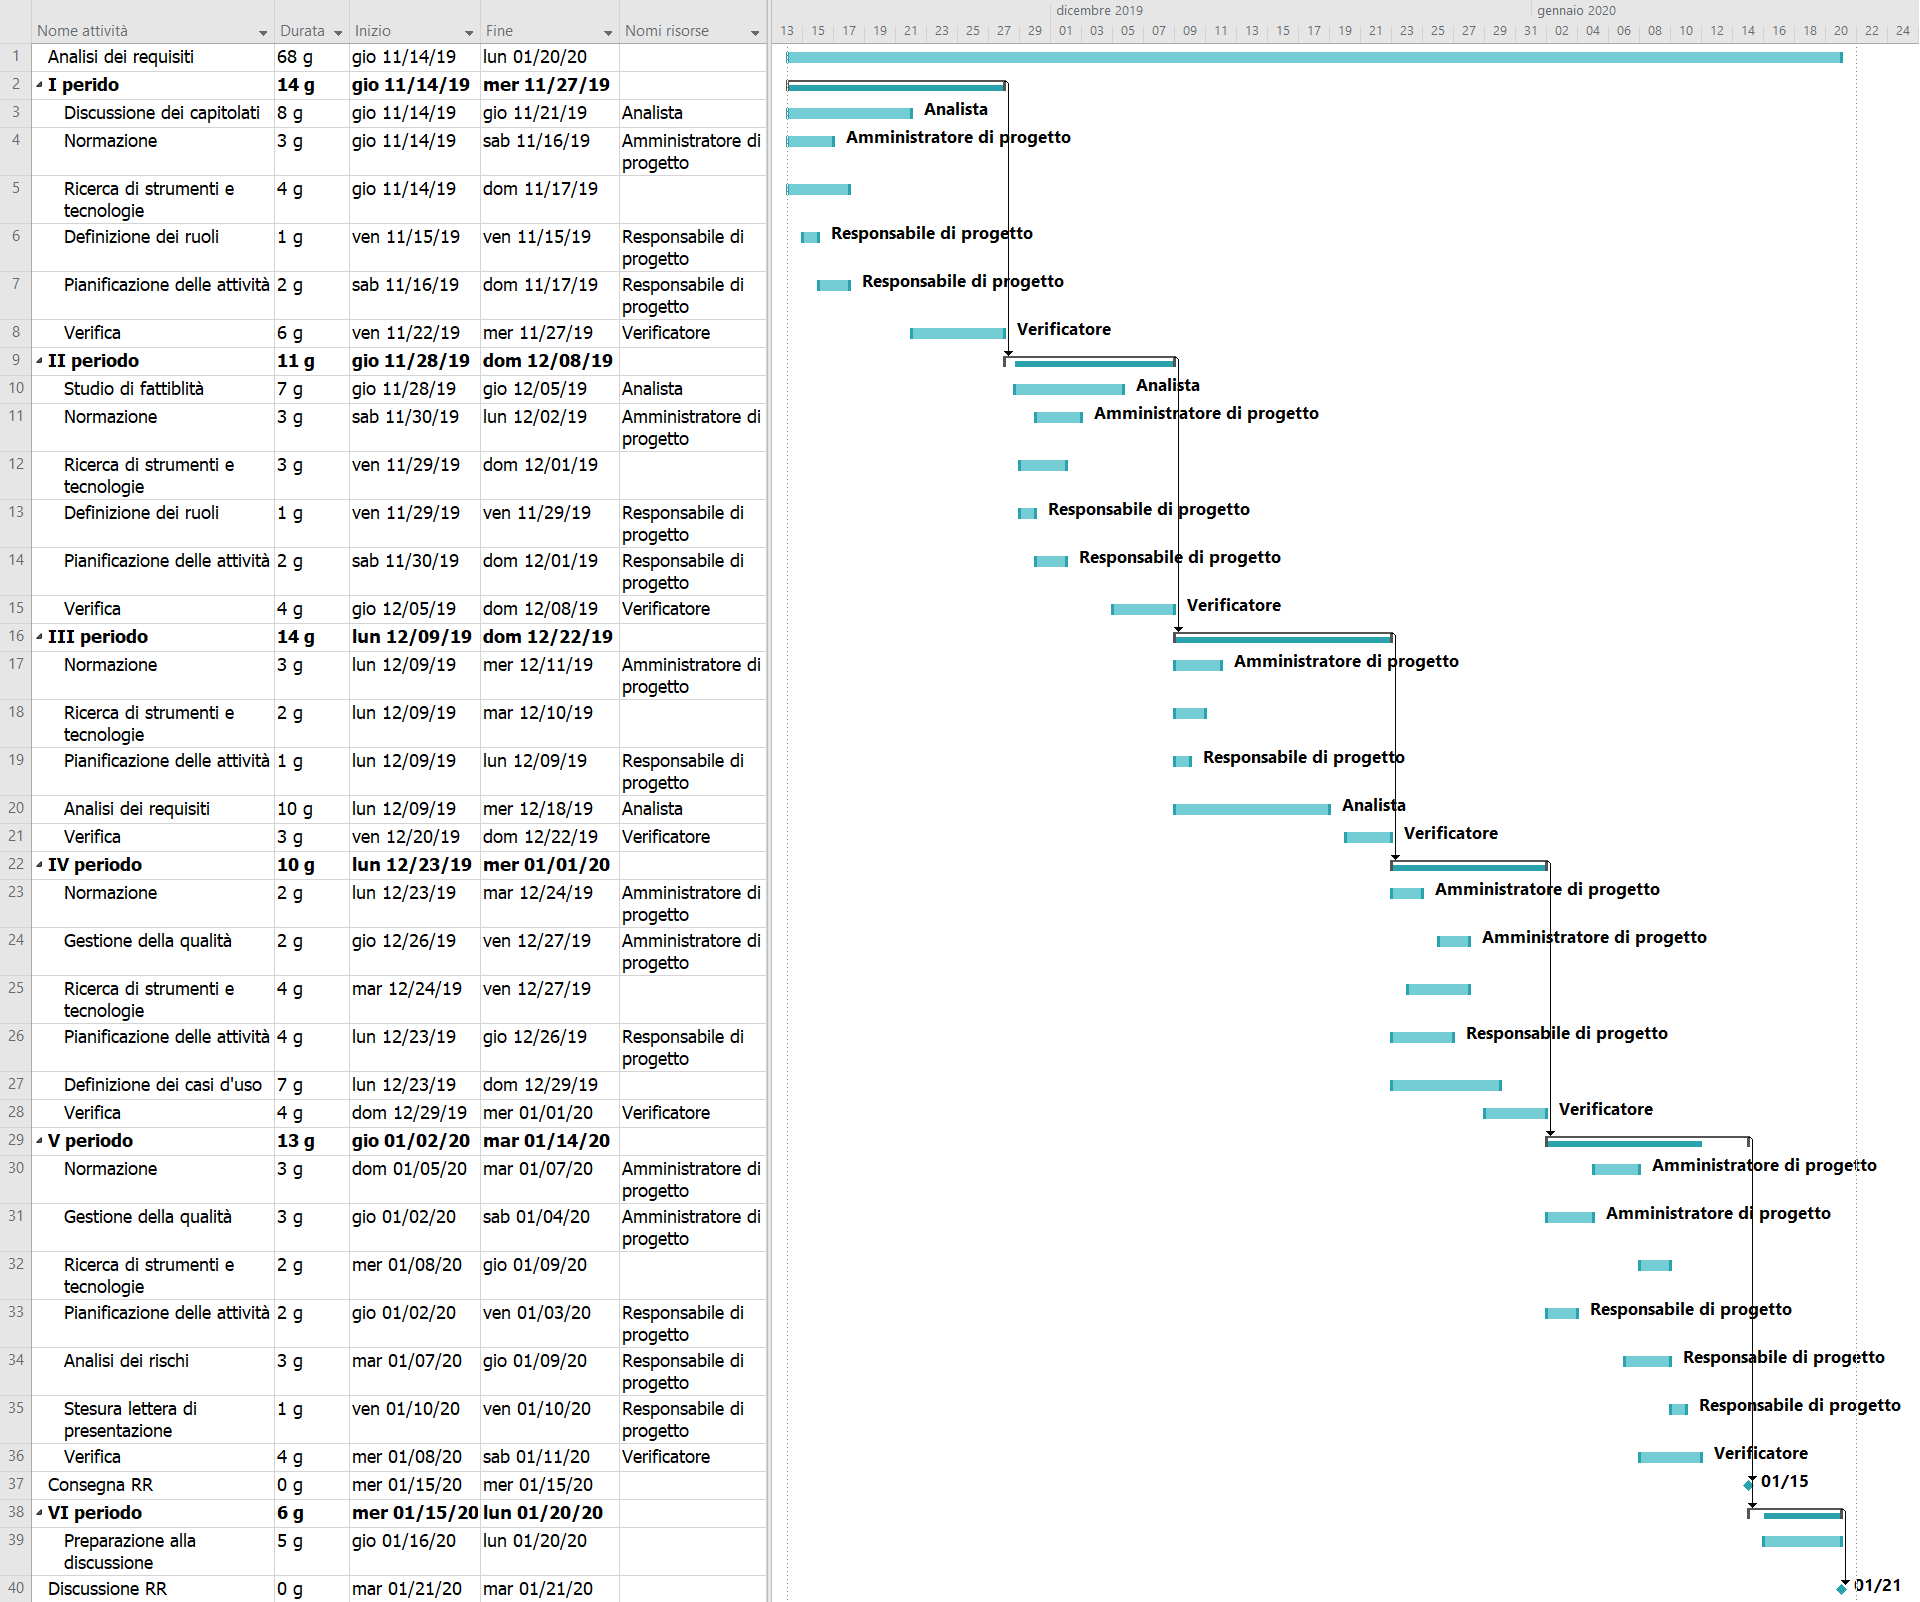
\includegraphics[width=\linewidth]{./gantt/Analisi dei requisiti.png}
	\caption{Diagramma di Gantt del periodo Analisi dei Requisiti}
\end{figure}
\pagebreak

\subsection{Progettazione architetturale}
La progettazione\glosp architetturale è il secondo macro periodo: inizia il 2020-01-22, giorno successivo alla prima revisione e finisce il 2020-02-20, giorno precedente alla seconda revisione. Durante questo macro periodo ci occuperemo della progettazione\glosp della codifica del codice del prodotto\glo.

\subsubsection{Ruoli attivi}
\begin{itemize}
	\item Responsabile di progetto\glo;
	\item amministratore di progetto\glo;
	\item analista;
	\item progettista;
	\item programmatore;
	\item verificatore.
\end{itemize}

\subsubsection{Periodi}
\paragraph*{I periodo: dal 2020-01-22 al 2020-02-09}
\begin{itemize}
	\item \textbf{Pianificazione delle attività}: gestione delle risorse disponibili, suddivisione e pianificazione di tutte le attività che devono essere svolte in questo periodo;
	\item \textbf{Normazione}: revisione e, se necessario, aggiornamento delle \textit{Norme di Progetto};
	\item \textbf{Gestione della qualità}: revisione delle metodologie per mantenere e garantire la qualità del prodotto\glo;
	\item \textbf{Revisione dei requisiti}: revisione ed, eventualmente, modifica dei requisiti analizzati durante la prima attività in seguito a modifiche di casi d'uso\glosp o di altre indicazioni;
	\item \textbf{Ricerca di strumenti e tecnologie}: ricerca delle tecnologie necessarie allo sviluppo del progetto\glo;
	\item \textbf{Verifica}: attività di controllo dei documenti modificati durante questo periodo.
\end{itemize}

\paragraph*{II periodo: dal 2020-02-10 al 2020-02-18}
\begin{itemize}
	\item \textbf{Pianificazione delle attività}: gestione delle risorse disponibili, suddivisione e pianificazione di tutte le attività che devono essere svolte in questo periodo;
	\item \textbf{Normazione}: revisione e aggiornamento delle \textit{Norme di Progetto};
	\item \textbf{Gestione della qualità}: revisione delle metodologie per mantenere e garantire la qualità del prodotto\glo;
	\item \textbf{Configurazione di strumenti e tecnologie}: configurazione delle tecnologie necessarie allo sviluppo del progetto\glo;
	\item \textbf{Revisione dei casi d'uso}\glo: revisione e modifica dei casi d'uso\glosp in seguito a indicazioni da parte del proponente;
	\item \textbf{Revisione dei requisiti}: revisione e modifica dei requisiti analizzati durante la prima attività in seguito a modifiche di casi d'uso\glosp o di altre indicazioni;
	\item \textbf{Progettazione}\glosp\textbf{proof of concept}\glo: pianificazione dello sviluppo di una proof of concept\glosp per dimostrare la fattibilità del prodotto\glo;
	\item \textbf{Verifica}: attività di controllo dei documenti modificati durante questo periodo.
\end{itemize}

\paragraph*{III periodo: dal 2020-02-19 al 2020-02-21}
\begin{itemize}
	\item \textbf{Normazione}: revisione e aggiornamento delle \textit{Norme di Progetto};
	\item \textbf{Pianificazione delle attività}: gestione delle risorse disponibili, suddivisione e pianificazione di tutte le attività che devono essere svolte in questo periodo;
	\item \textbf{Codifica proof of concept}\glo: sviluppo del codice per realizzare il proof of concept\glosp precedentemente pianificato, implementazione degli incrementi 1 e 9 del modello di sviluppo incrementale;
	\item \textbf{Stesura lettera di presentazione}: stesura della \textit{Lettera di Presentazione} in cui si propone una soluzione alla richiesta del proponente;
	\item \textbf{Verifica}: attività di controllo dei documenti e del codice sorgente realizzati durante questo periodo.
\end{itemize}

\paragraph*{IV periodo: dal 2020-02-22 al 2020-02-25}
\begin{itemize}
	\item \textbf{Pianificazione delle attività}: gestione delle risorse disponibili, suddivisione e pianificazione di tutte le attività che devono essere svolte in questo periodo;
	% Verificare se scrivere incremento 7 e 15 come parziali: nel PoC faremo solo esportazione del file e visualizzazione dei dati
	% Da incremento 7 eventualmente togliere "creazione"
	% Da incremento 15 eventualmente togliere "elaborazione"
	\item \textbf{Codifica proof of concept}\glo: sviluppo del codice per realizzare il proof of concept\glosp precedentemente pianificato, implementazione degli incrementi 2, 7, 12 e 15 del modello di sviluppo incrementale;
	\item \textbf{Verifica}: attività di controllo dei documenti e del codice sorgente realizzati durante questo periodo.
\end{itemize}

\paragraph*{V periodo: dal 2020-02-26 al 2020-03-08}
\begin{itemize}
	\item \textbf{Studio di strumenti e tecnologie}: revisione delle tecnologie e degli strumenti necessari per lo sviluppo del prodotto\glosp richiesto dal proponente in seguito alla presentazione dei PoC\glosp agli stakeholder\glo;
	\item \textbf{Normazione}: revisione e aggiornamento delle \textit{Norme di Progetto};
	\item \textbf{Pianificazione delle attività}: gestione delle risorse disponibili, suddivisione e pianificazione di tutte le attività che devono essere svolte in questo periodo;
	\item \textbf{Progettazione}\glosp\textbf{proof of concept}\glo: eventuale revisione della progettazione\glosp della proof of concept\glosp per dimostrare la fattibilità del prodotto\glo;
	\item \textbf{Codifica proof of concept}\glo: aggiornamento del codice del proof of concept\glosp in seguito alla presentazione agli stakeholder\glo;
	\item \textbf{Stesura lettera di presentazione}: stesura della \textit{Lettera di Presentazione} in cui si propone una soluzione alla richiesta del proponente;
	\item \textbf{Verifica}: attività di controllo dei documenti e del codice sorgente realizzati durante questo periodo.
\end{itemize}

\paragraph*{VI periodo: dal 2020-03-09 al 2020-03-15}
\begin{itemize}
	\item \textbf{Preparazione alla discussione}: realizzazione della presentazione e preparazione individuale e di gruppo alla discussione.
\end{itemize}

\begin{landscape}
	\begin{figure}
		\centering
		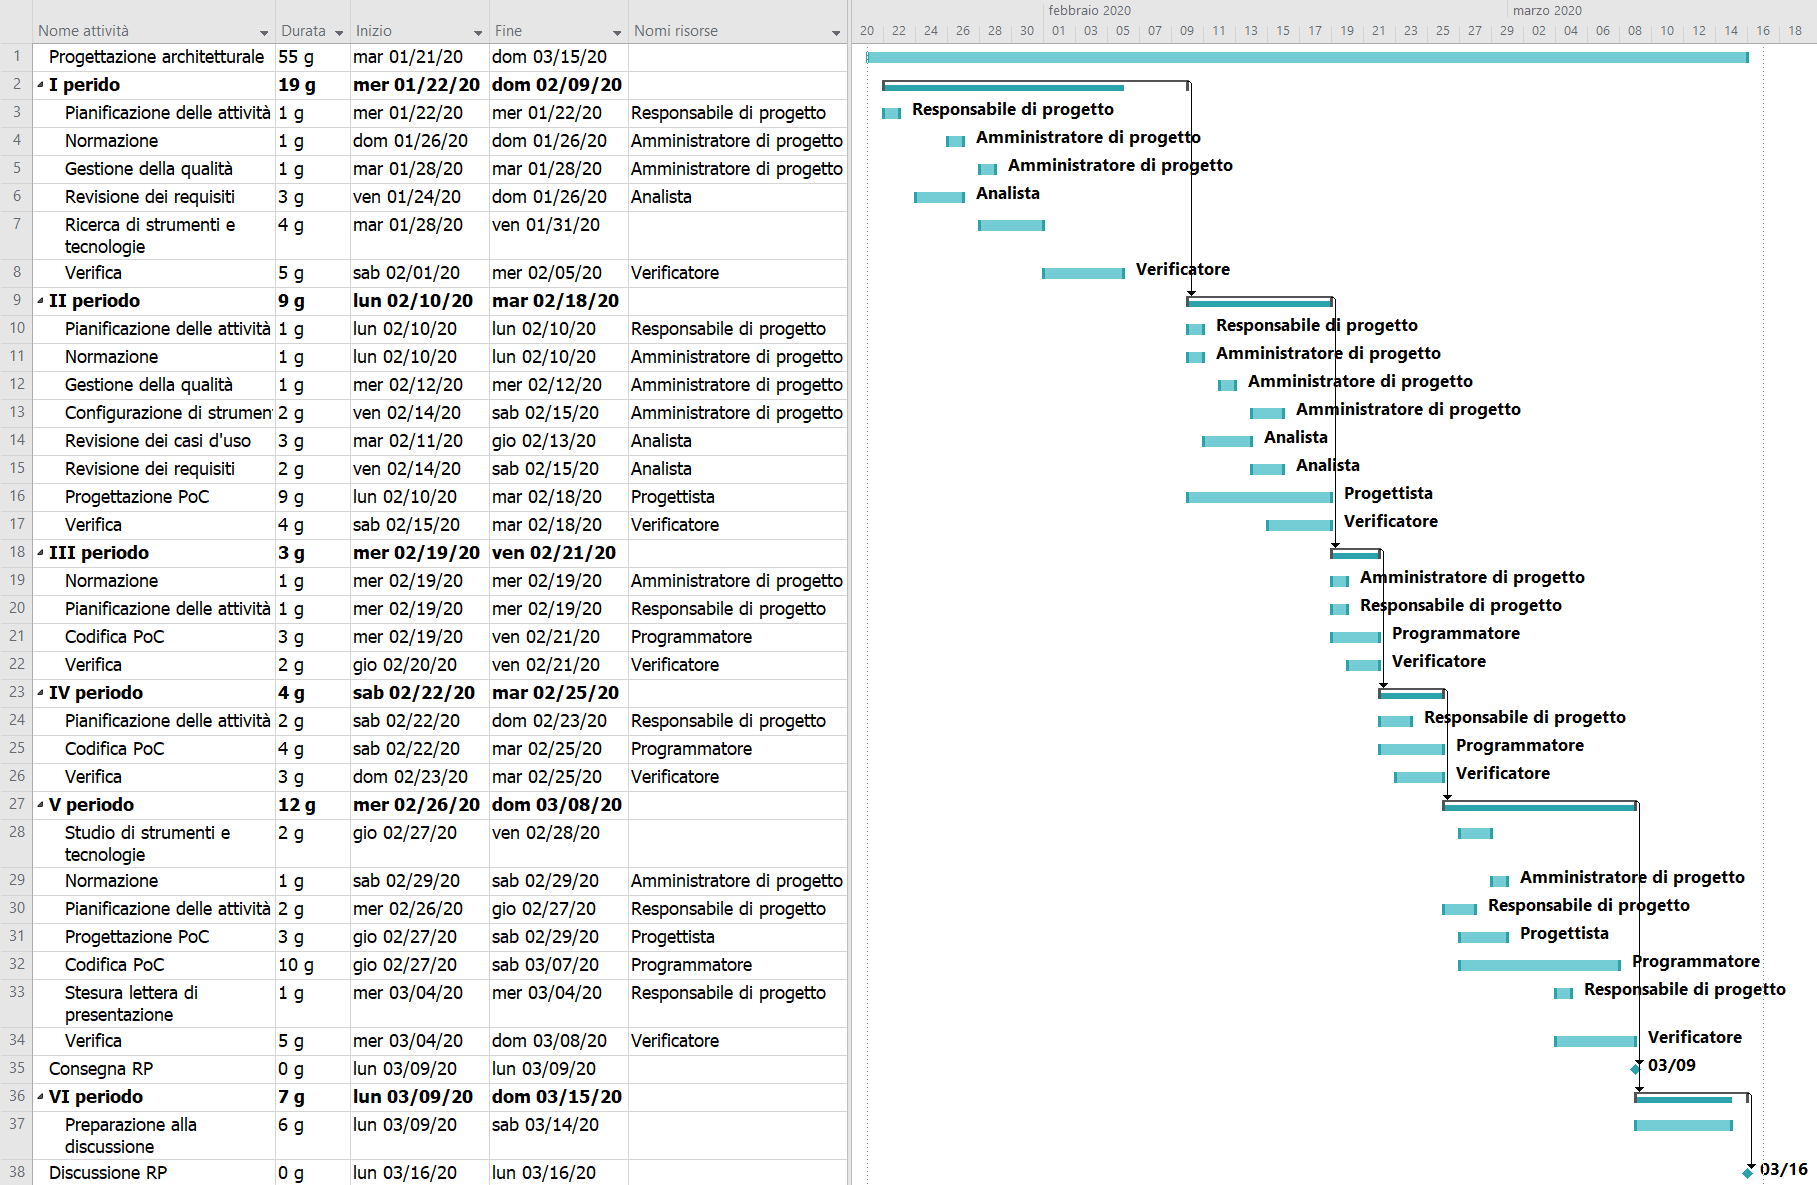
\includegraphics[scale=0.512]{./gantt/Progettazione architetturale.png}
		\caption{Diagramma di Gantt del periodo Progettazione Architetturale}
	\end{figure}
\end{landscape}
\pagebreak


\subsection{Progettazione di dettaglio e codifica}
La progettazione\glosp di dettaglio e codifica è il nostro terzo macro periodo: inizia il 2020-03-17, giorno successivo alla seconda revisione e finisce il 2020-04-19, giorno precedente alla terza revisione. Durante questo periodo ci occuperemo principalmente dell'attività di progettazione di dettaglio e di codifica del prodotto\glo. \\
In particolare ci poniamo i seguenti obiettivi:
\begin{itemize}
	\item revisione e aggiornamento dei documenti;
	\item revisione e aggiornamento della progettazione architetturale del prodotto\glosp software;
	\item definizione dell'architettura di dettaglio del prodotto\glosp software;
	\item stesura dell'allegato tecnico alla Product Baseline\glo;
	\item stesura del \textit{Manuale dello sviluppatore};
	\item implementazione degli incrementi necessari a garantire la presenza delle funzionalità fondamentali del prodotto. In particolare:
		\begin{itemize}
		\item incremento 3;
		\item incremento 4;
		\item incremento 6;
		\item incremento 13;
		\item incremento 14;
		\item incremento 16.
		\end{itemize}
	\item verifica di quanto implementato;
	\item stesura del \textit{Manuale Utente} sulla base degli incrementi sviluppati;
	\item conseguimento del colloquio per la Product Baseline\glosp con il committente;
	\item realizzazione della presentazione e preparazione alla discussione.
\end{itemize}
Al termine di questo periodo ci aspettiamo quindi di avere un prodotto\glosp di qualità che fornisca le funzionalità fondamentali e con un livello di copertura dei test accettabile. 
\subsubsection*{Ruoli attivi}
\begin{itemize}
	\item Responsabile di progetto\glo;
	\item amministratore di progetto\glo;
	\item analista;
	\item progettista;
	\item programmatore;
	\item verificatore.
\end{itemize}
Di seguito analizziamo la pianificazione di dettaglio per quanto concerne lo sviluppo di ciascun incremento.

\subsubsection{Incremento 3}
\textbf{I periodo: dal 2020-03-17 al 2020-03-24} \\ 
L'incremento 3 prevede lo sviluppo e l'implementazione dell'algoritmo di addestramento SVM\glosp nell'applicazione di addestramento e nel plug-in. 
\\Prevede il soddisfacimento completo o parziale dei seguenti requisiti:
\begin{itemize}
	\item R1F4.2;
	\item R1F4.10;
	\item R1F11;
	\item R2F4.6.
\end{itemize}
Viene svolto in un unico periodo.
\paragraph{Ruoli attivi}
\begin{itemize}
	\item Responsabile di progetto\glo;
	\item amministratore di progetto\glo;
	\item analista
	\item progettista;
	\item programmatore;
	\item verificatore.
\end{itemize}
\paragraph{Attività} 
\begin{itemize}
	\item \textbf{Revisione dei documenti}: revisione e, se necessario, aggiornamento dei documenti secondo le indicazioni del committente;
	\item \textbf{Normazione}: revisione e, se necessario, aggiornamento delle \textit{Norme di Progetto};
	\item \textbf{Ricerca di strumenti e tecnologie}: ricerca e studio degli strumenti e tecnologie utilizzate per la codifica;
	\item \textbf{Pianificazione delle attività}: gestione delle risorse disponibili, suddivisione e pianificazione di tutte le attività che devono essere svolte in questo periodo;
	\item \textbf{Progettazione}\glo: definizione in modo più dettagliato ed eventuali correzioni dell'architettura del nostro prodotto\glosp software con rispettiva individuazione dei design pattern architetturali da applicare e progettazione\glosp dell'incremento 3; 
	\item \textbf{Revisione dei requisiti}: revisione ed, eventualmente, modifica dei requisiti analizzati secondo le indicazioni; 
	\item \textbf{Codifica}: scrittura del codice del prodotto\glosp seguendo le indicazioni definite nel documento \textit{Norme di Progetto} e nella progettazione\glosp indicata sopra. Codifica per l'implementazione dell'incremento 3; 
	\item \textbf{Verifica}: attività di controllo dei documenti e del codice realizzati durante questo periodo.
\end{itemize}
\subsubsection{Incremento 4}
\textbf{II periodo: dal 2020-03-25 al 2020-03-30} \\
L'incremento 4 prevede lo sviluppo e l'implementazione dell'algoritmo di addestramento RL\glosp nell'applicazione di addestramento e nel plug-in.
\\Prevede il soddisfacimento completo o parziale dei seguenti requisiti:
\begin{itemize}
	\item R1F4.2;
	\item R1F4.11. 
\end{itemize}
Viene svolto in un unico periodo.
\paragraph{Ruoli attivi}
\begin{itemize}
	\item Responsabile di progetto\glo;
	\item amministratore di progetto\glo;
	\item analista
	\item progettista;
	\item programmatore;
	\item verificatore.
\end{itemize}
\paragraph{Attività} 
\begin{itemize}
	\item \textbf{Normazione}: revisione e, se necessario, aggiornamento delle \textit{Norme di Progetto};
	\item \textbf{Ricerca di strumenti e tecnologie}: ricerca e studio degli strumenti e tecnologie utilizzate per la codifica;
	\item \textbf{Pianificazione delle attività}: gestione delle risorse disponibili, suddivisione e pianificazione di tutte le attività che devono essere svolte in questo periodo;
	\item \textbf{Progettazione}\glo: revisione e aggiornamento della progettazione\glosp dell'architettura del prodotto\glosp con rispettiva individuazione dei design pattern architetturali da applicare e progettazione\glosp dell'incremento 4; 
	\item \textbf{Revisione dei requisiti}: revisione ed, eventualmente, modifica dei requisiti analizzati secondo le indicazioni; 
	\item \textbf{Codifica}: scrittura del codice del prodotto\glosp seguendo le indicazioni definite nel documento \textit{Norme di Progetto} e nella progettazione\glosp indicata sopra. Codifica per l'implementazione dell'incremento 4;
	\item \textbf{Scrittura manuale sviluppatore}: inizio della scrittura del \textit{Manuale dello sviluppatore} per fornire le indicazioni utili ad uno sviluppatore che vuole contribuire al progetto\glo; 
	\item \textbf{Verifica}: attività di controllo dei documenti e del codice realizzati durante questo periodo.
\end{itemize}
\subsubsection{Incremento 6}
\textbf{III periodo: dal 2020-03-31 al 2020-04-02} \\
L'incremento 6 prevede lo sviluppo e l'implementazione della funzionalità che permette all'utente di selezionare un modello di predizione e avviare l'addestramento dello stesso.
\\Prevede il soddisfacimento completo o parziale dei seguenti requisiti:
\begin{itemize}
	\item R1F4.4;
	\item R1F4.11;
	\item R1F4.12.
\end{itemize}
Viene svolto in un unico periodo.
\paragraph{Ruoli attivi}
\begin{itemize}
	\item Responsabile di progetto\glo;
	\item amministratore di progetto\glo;
	\item progettista;
	\item programmatore;
	\item verificatore.
\end{itemize}
\paragraph{Attività} 
\begin{itemize}
	\item \textbf{Normazione}: revisione e, se necessario, aggiornamento delle \textit{Norme di Progetto};
	\item \textbf{Ricerca di strumenti e tecnologie}: ricerca e studio degli strumenti e tecnologie utilizzate per la codifica;
	\item \textbf{Pianificazione delle attività}: gestione delle risorse disponibili, suddivisione e pianificazione di tutte le attività che devono essere svolte in questo periodo;
	\item \textbf{Progettazione}\glo: progettazione\glosp dell'incremento 6;  
	\item \textbf{Codifica}: scrittura del codice del prodotto\glosp seguendo le indicazioni definite nel documento \textit{Norme di Progetto} e nella progettazione\glosp indicata sopra. Codifica per l'implementazione dell'incremento 6;
	\item \textbf{Scrittura manuale sviluppatore}: aggiornamento del \textit{Manuale dello sviluppatore};
	\item \textbf{Verifica}: attività di controllo dei documenti e del codice realizzati durante questo periodo.
\end{itemize}
\subsubsection{Incremento 13}
\textbf{IV periodo: dal 2020-04-03 al 2020-04-05} \\
L'incremento 13 prevede lo sviluppo e l'implementazione della lettura del file di configurazione, che sarà in formato JSON, e la conseguente configurazione degli algoritmi.
\\Prevede il soddisfacimento completo o parziale dei seguenti requisiti:
\begin{itemize}
	\item R1F8;
	\item R1F11.
\end{itemize}
Viene svolto in un unico periodo.
\paragraph{Ruoli attivi}
\begin{itemize}
	\item Responsabile di progetto\glo;
	\item amministratore di progetto\glo;
	\item progettista;
	\item programmatore;
	\item verificatore.
\end{itemize}
\paragraph{Attività} 
\begin{itemize}
	\item \textbf{Normazione}: revisione e, se necessario, aggiornamento delle \textit{Norme di Progetto};
	\item \textbf{Pianificazione delle attività}: gestione delle risorse disponibili, suddivisione e pianificazione di tutte le attività che devono essere svolte in questo periodo;
	\item \textbf{Progettazione}\glo: progettazione\glosp dell'incremento 13;  
	\item \textbf{Codifica}: scrittura del codice del prodotto\glosp seguendo le indicazioni definite nel documento \textit{Norme di Progetto} e nella progettazione\glosp indicata sopra. Codifica per l'implementazione dell'incremento 13;
	\item \textbf{Scrittura manuale sviluppatore}: aggiornamento del \textit{Manuale dello sviluppatore};
	\item \textbf{Scrittura manuale utente}: inizio della scrittura del \textit{Manuale utente} per descrivere come deve l'utente finale deve utilizzare il software;
	\item \textbf{Verifica}: attività di controllo dei documenti e del codice realizzati durante questo periodo.
\end{itemize}
\subsubsection{Incremento 14}
\textbf{V periodo: dal 2020-04-06 al 2020-04-10} \\
L'incremento 14 prevede lo sviluppo e l'implementazione dell'associazione dei nodi al flusso dati e dell'elaborazione e visualizzazione dei dati.
\\Prevede il soddisfacimento completo o parziale dei seguenti requisiti:
\begin{itemize}
	\item R1F9;
	\item R1F9.1;
	\item R1F9.2;
	\item R1F9.4;
	\item R1F9.5;
	\item R1F11.
\end{itemize}
Viene svolto in un unico periodo.
\paragraph{Ruoli attivi}
\begin{itemize}
	\item Responsabile di progetto\glo;
	\item amministratore di progetto\glo;
	\item progettista;
	\item programmatore;
	\item verificatore.
\end{itemize}
\paragraph{Attività} 
\begin{itemize}
	\item \textbf{Normazione}: revisione e, se necessario, aggiornamento delle \textit{Norme di Progetto};
	\item \textbf{Pianificazione delle attività}: gestione delle risorse disponibili, suddivisione e pianificazione di tutte le attività che devono essere svolte in questo periodo;
	\item \textbf{Progettazione}\glo: progettazione\glosp dell'incremento 14;  
	\item \textbf{Codifica}: scrittura del codice del prodotto\glosp seguendo le indicazioni definite nel documento \textit{Norme di Progetto} e nella progettazione\glosp indicata sopra. Codifica per l'implementazione dell'incremento 14;
	\item \textbf{Scrittura manuale sviluppatore}: aggiornamento del \textit{Manuale dello sviluppatore};
	\item \textbf{Scrittura manuale utente}: aggiornamento del \textit{Manuale utente};
	\item \textbf{Verifica}: attività di controllo dei documenti e del codice realizzati durante questo periodo.
\end{itemize}
\subsubsection{Incremento 16}
\textbf{VI periodo: dal 2020-04-11 al 2020-04-13} \\
L'incremento 16 prevede lo sviluppo e l'implementazione della funzionalità che permette all'utente di arrestare l'algoritmo di addestramento prima del suo termine naturale.
\\Prevede il soddisfacimento completo o parziale dei seguenti requisiti:
\begin{itemize}
	\item R1F12;
	\item R1F20.
\end{itemize}
Viene svolto in un unico periodo.
\paragraph{Ruoli attivi}
\begin{itemize}
	\item Responsabile di progetto\glo;
	\item amministratore di progetto\glo;
	\item progettista;
	\item programmatore;
	\item verificatore.
\end{itemize}
\paragraph{Attività} 
\begin{itemize}
	\item \textbf{Normazione}: revisione e, se necessario, aggiornamento delle \textit{Norme di Progetto};
	\item \textbf{Pianificazione delle attività}: gestione delle risorse disponibili, suddivisione e pianificazione di tutte le attività che devono essere svolte in questo periodo;
	\item \textbf{Progettazione}\glo: progettazione\glosp dell'incremento 16;  
	\item \textbf{Codifica}: scrittura del codice del prodotto\glosp seguendo le indicazioni definite nel documento \textit{Norme di Progetto} e nella progettazione\glosp indicata sopra. Codifica per l'implementazione dell'incremento 16;
	\item \textbf{Scrittura manuale sviluppatore}: chiusura del \textit{Manuale dello sviluppatore};
	\item \textbf{Scrittura manuale utente}: chiusura del \textit{Manuale utente};
	\item \textbf{Stesura lettera di presentazione}: stesura della \textit{Lettera di Presentazione} in cui si propone una soluzione alla richiesta del proponente;
	\item \textbf{Verifica}: attività di controllo dei documenti e del codice realizzati durante questo periodo.
\end{itemize}
\subsubsection{VII periodo: dal 2020-04-14 al 2020-04-19}
Durante questo periodo è prevista la preparazione alla discussione della revisione di qualifica.
\paragraph{Ruoli attivi} \mbox{}\\ [1mm]
Non è previsto alcun ruolo attivo.
\paragraph{Attività}

\begin{itemize}
	\item \textbf{Preparazione alla discussione}: realizzazione della presentazione e preparazione individuale e di gruppo alla discussione.
\end{itemize}

\begin{figure}
	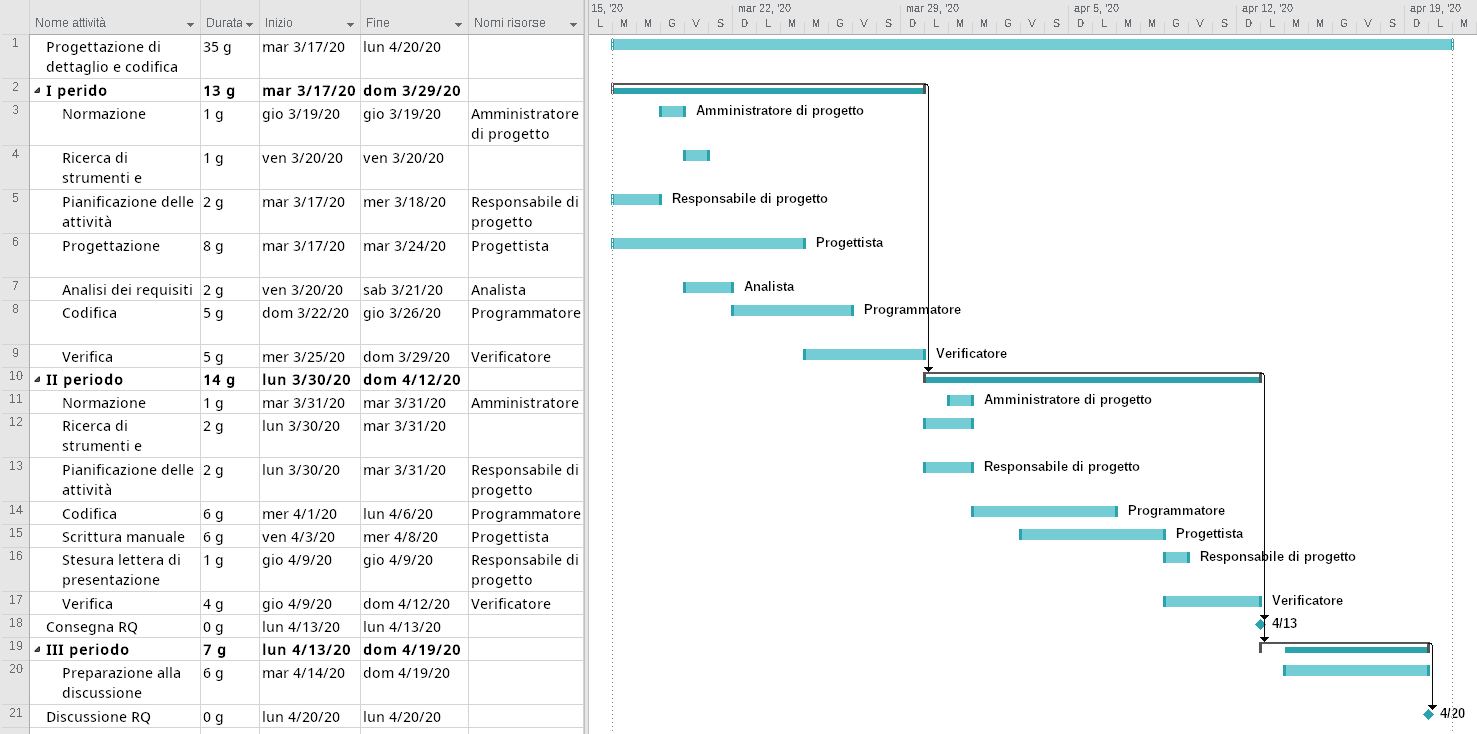
\includegraphics[width=\linewidth]{./gantt/Progettazione di dettaglio e codifica.png}
	\caption{Diagramma di Gantt del periodo Progettazione di dettaglio e codifica}
\end{figure}
\pagebreak

\subsection{Validazione e collaudo}
Validazione\glosp e collaudo è il nostro quarto macro periodo: inizia il 2020-04-21, giorno successivo alla terza revisione e si conclude il 2020-05-17, giorno precedente all'ultima revisione. Durante questo macro periodo ci occuperemo dello sviluppo di due incrementi che completano il nostro prodotto e del collaudo e della validazione\glosp dello stesso. per verificare che tutti i requisiti definiti come obbligatori nell'\textit{Analisi dei Requisiti} siano stati soddisfatti. \\
In particolare per questo periodo ci poniamo i seguenti obiettivi:
\begin{itemize}
	\item revisione e aggiornamento dei documenti;	
	\item implementazione degli incrementi rimanenti per completare le funzionalità del prodotto\glosp previste. In particolare:
		\begin{itemize}
			\item incremento 8;
			\item incremento 17.
		\end{itemize}
	\item verifica di quanto implementato;
	\item aggiornamento del \textit{Manuale dello sviluppatore};
	\item aggiornamento del \textit{Manuale Utente};
	\item realizzazione della presentazione e preparazione alla discussione.	
\end{itemize}
Al termine di questo periodo ci aspettiamo quindi di avere un prodotto\glosp di qualità completo, con un livello di copertura dei test accettabile e approvato dal proponente. 

\subsubsection*{Ruoli attivi}
\begin{itemize}
	\item Responsabile di progetto\glo;
	\item amministratore di progetto\glo;
	\item progettista;
	\item programmatore;
	\item verificatore.
\end{itemize}

Di seguito analizziamo la pianificazione di dettaglio per quanto concerne lo sviluppo di ciascun incremento e le attività di correzione e chiusura finale dei documenti.

\subsubsection{Incremento 8}
\textbf{I periodo: dal 2020-04-21 al 2020-04-28} \\
L'incremento 8 prevede lo sviluppo e l'implementazione della funzionalità di visualizzazione degli indici di qualità dell'addestramento degli algoritmi.
\\Prevede il soddisfacimento completo o parziale dei seguenti requisiti:
\begin{itemize}
	\item R1F5;
	\item R1F5.1;
	\item R1F5.2;
	\item R1F5.3.
\end{itemize}
Viene svolto in un unico periodo.
\paragraph{Ruoli attivi}
\begin{itemize}
	\item Responsabile di progetto\glo;
	\item amministratore di progetto\glo;
	\item progettista;
	\item programmatore;
	\item verificatore.
\end{itemize}
\paragraph{Attività}
\begin{itemize}
	\item \textbf{Normazione}: revisione e, se necessario, aggiornamento delle \textit{Norme di Progetto};
	\item \textbf{Pianificazione delle attività}: gestione delle risorse disponibili, suddivisione e pianificazione di tutte le attività che devono essere svolte in questo periodo;
	\item \textbf{Progettazione}: progettazione di dettaglio dell'incremento 8;
	\item \textbf{Codifica}: implementazione dell'incremento 8 seguendo le indicazioni delle \textit{Norme di Progetto} e della progettazione\glosp indicata sopra;
	\item \textbf{Test e collaudo}: scrittura dei test mancanti per il collaudo finale del prodotto\glo;
	\item \textbf{Verifica}: attività di controllo del codice e dei documenti realizzati durante questo periodo.
\end{itemize}

\subsubsection{Incremento 17}
\textbf{II periodo: dal 2020-04-29 al 2020-05-02} \\
L'incremento 17 prevede lo sviluppo e l'implementazione della funzionalità di visualizzazione degli errori in caso di inserimento di file non validi e errata mappatura dei predittori con il flusso di dati ricevuto dalla datasource.
\\Prevede il soddisfacimento completo o parziale dei seguenti requisiti:
\begin{itemize}
	\item R2F6;
	\item R2F10;
	\item R2F18.
\end{itemize}
Viene svolto in un unico periodo.
\paragraph{Ruoli attivi}
\begin{itemize}
	\item Responsabile di progetto\glo;
	\item amministratore di progetto\glo;
	\item progettista;
	\item programmatore;
	\item verificatore.
\end{itemize}
\paragraph{Attività}
\begin{itemize}
	\item \textbf{Normazione}: revisione e, se necessario, aggiornamento delle \textit{Norme di Progetto};
	\item \textbf{Pianificazione delle attività}: gestione delle risorse disponibili, suddivisione e pianificazione di tutte le attività che devono essere svolte in questo periodo;
	\item \textbf{Progettazione}: progettazione di dettaglio dell'incremento 17;
	\item \textbf{Manuale utente}: integrazione delle nuove funzionalità del prodotto\glo;
	\item \textbf{Manuale sviluppatore}:  revisione e, se necessario, aggiornamento del \textit{Manuale dello Sviluppatore};
	\item \textbf{Codifica}: implementazione dell'incremento 17 seguendo le indicazioni delle \textit{Norme di Progetto} e della progettazione\glosp indicata sopra;
	\item \textbf{Test e collaudo}: scrittura dei test mancanti per il collaudo finale del prodotto\glo;
	\item \textbf{Verifica}: attività di controllo del codice e dei documenti realizzati durante questo periodo.
\end{itemize}

\subsubsection{III periodo: dal 2020-05-03 al 2020-05-10}
Durante questo periodo è prevista la correzione e la chiusura di tutti i documenti.
\paragraph{Ruoli attivi}
\begin{itemize}
	\item Responsabile di progetto\glo;
	\item amministratore di progetto\glo;
	\item progettista;
	\item programmatore;
	\item verificatore.
\end{itemize}
\paragraph{Attività}
\begin{itemize}
	\item \textbf{Norme di progetto}: revisione e, se necessario, aggiornamento delle \textit{Norme di Progetto};
	\item \textbf{Pianificazione delle attività}: gestione delle risorse disponibili, suddivisione e pianificazione di tutte le attività che devono essere svolte in questo periodo;
	\item \textbf{Revisione dei documenti}: revisione e, se necessario, aggiornamento dei documenti secondo le indicazioni del committente;
	\item \textbf{Codifica}: codifica dei rimanenti test per il collaudo del prodotto\glosp ed eventuali bug fix;
	\item \textbf{Test e collaudo}: esecuzione finale dei test per il collaudo del prodotto\glo;
	\item \textbf{Verifica}: attività di controllo dei documenti e del codice realizzati durante questo periodo;
	\item \textbf{Stesura lettera di presentazione}: stesura della \textit{Lettera di Presentazione} che in cui si propone una soluzione alla richiesta del proponente.
\end{itemize}

\subsubsection{IV periodo: dal 2020-05-11 al 2020-05-17}
Durante questo periodo è prevista la preparazione alla discussione finale.
\paragraph{Ruoli attivi} \mbox{}\\ [1mm]
Non è previsto alcun ruolo attivo.
\paragraph{Attività}

\begin{itemize}
	\item \textbf{Preparazione alla discussione}: realizzazione della presentazione e preparazione individuale e di gruppo alla discussione.
\end{itemize}

\begin{landscape}
	\begin{figure}
		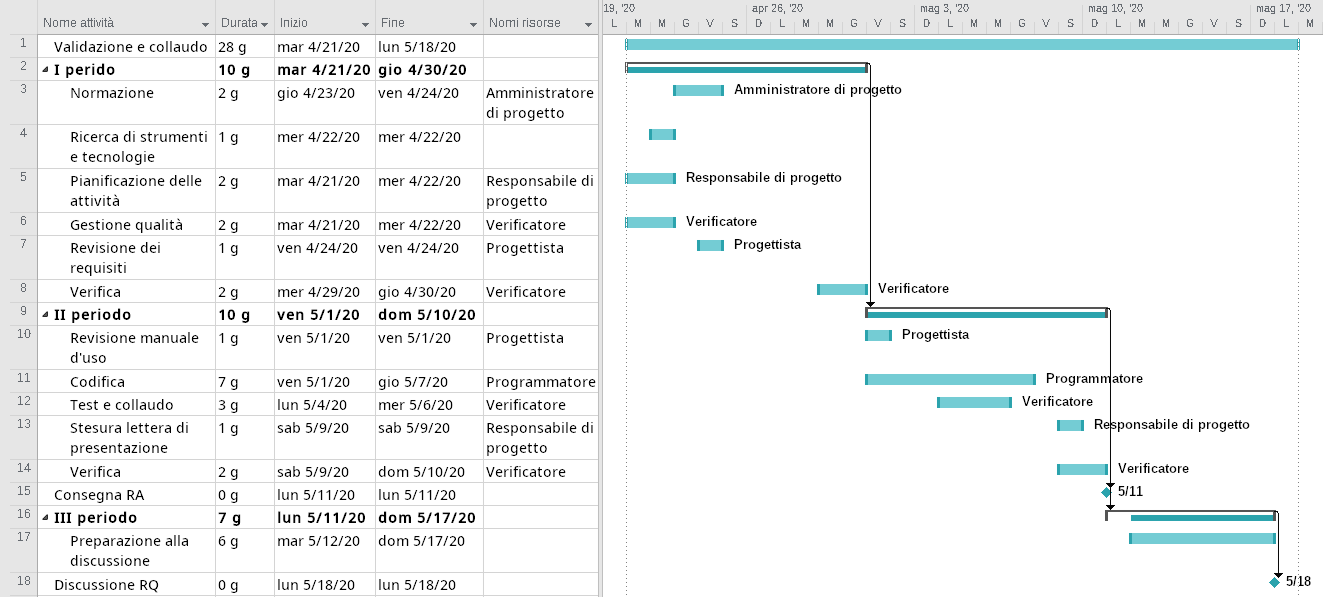
\includegraphics[width=\linewidth]{./gantt/Validazione e collaudo.png}
		\caption{Diagramma di Gantt del periodo Validazione e collaudo}
	\end{figure}
\end{landscape}
\pagebreak
 
	
	
	
	%Input del file "decision_table" della cartella locale "res/"
	% \textbf = grassetto; \Large = font più grande
% \rowcolors{quanti colori alternare}{colore numero riga pari}{colore numero riga dispari}: colori alternati per riga
% \rowcolor{color}: cambia colore di una riga
% p{larghezza colonna}: p è un tipo di colonna di testo verticalmente allineata sopra, ci sarebbe anche m che è centrata a metà ma non è precisa per questo utilizzo TBStrut; la sintassi >{\centering} indica che il contenuto della colonna dovrà essere centrato
% \TBstrut fa parte di alcuni comandi che ho inserito in config.tex che permetto di aggiungere un po' di padding al testo
% \\ [2mm] : questra scrittura indica che lo spazio dopo una break line deve essere di 2mm

%\setcounter{secnumdepth}{0}
%\hfill \break
%\textbf{\Large{Diario delle modifiche}} \\
\section{Riepilogo tracciamenti}
\rowcolors{2}{gray!25}{gray!15}
\begin{longtable} {
		>{\centering}p{17mm} 
		%>{\centering}p{19.5mm}
		%>{\centering}p{24mm} 
		%>{\centering}p{24mm} 
		>{}p{120mm}}
	\rowcolor{gray!50}
	\textbf{Codice} & \multicolumn{1}{c}{\textbf{Decisione}} \\%\textbf{Decisione} \\ %\TBstrut \\
	VI\_1.1 & Scelto \textit{VRAM Software} come nome del gruppo. \TBstrut \\ [2mm]
	VI\_1.1 & Scelto \textit{VRAM Software} come nome del gruppo. \TBstrut \\ [2mm]
	VI\_1.1 & Scelto \textit{VRAM Software} come nome del gruppo. \TBstrut \\ [2mm]
	
\end{longtable} %Tabella delle decisioni (solo per i verbali)
\end{document}